\chapter{He Turned \$100k Into \$25M}

This School of Hard Knocks interview, curated by LazyingArt LLC, is not a blackboard lecture in the usual sense. Its mathematics is commercial rather than formal: the lecture moves from earned income to owned cash flow, from vague ambition to concrete deal structure, and from the myth of capital scarcity to the stronger claim that good deals are the truly scarce object. We therefore keep close to the transcript, preserve the order in which the ideas appear, and make the numerical spine explicit without pretending that the speaker supplied more detail than he did.

\section{Opening Claims and the Problem of Durable Wealth}

The lecture begins by compressing an entire entrepreneurial biography into a few hard markers: Miami, a first property bought at twenty-five, a bank account driven nearly to zero, a present-day business of large scale, and an order-of-magnitude claim about the portfolio. The point of this opening is not merely praise. It is to tell us that the speaker has already crossed the terrain that the rest of the lecture will try to map.

\begin{figure}[h]
\centering

\includegraphics[width=0.82\textwidth]{lecture_110_figure_02.png}
\caption{Opening visual emphasis on the scale claim: an eight-figure real-estate portfolio.}
\end{figure}

We should note the discipline of that first visual claim. The frame gives an order of magnitude and no more. It tells us that the portfolio is in the eight-figure range, but it does not supply an audited number, a leverage ratio, or a balance-sheet decomposition. In the notes we therefore preserve the scale claim without sharpening it beyond what the lecture shows.

The first economic move of the lecture is then easy to state. Napola wants to leave a world in which income is tied directly to transactional activity and move toward a structure in which the owned asset itself throws off income. In a compact notation, the contrast begins here:
\begin{equation}
I_{\text{comm}} \propto N_{\text{trades}},
\qquad
N_{\text{trades}} = 0 \Rightarrow I_{\text{comm}} = 0.
\end{equation}
This is not a financial model in full dress. It is the lecture's first governing relation: if the trades stop, the commissions stop. The rest of the chapter asks what sort of ownership structure loosens that dependence.

\section{Mentorship as an Accelerator}

After the opening credentialing, the lecture pivots immediately into advice to the younger self. The answer is crisp: find a mentor. This appears early because the speaker wants to define leverage before he discusses money. In the lecture, the first thing that compounds is not capital. It is access to a better operator's pattern of thought.

The Gary Rappaport episode gives the abstract instruction its mechanism. Napola hears a strong talk at a real-estate convention, notices that the speaker publicly offers his card, and then takes that offer seriously rather than romantically. He does not merely admire the speaker. He waits, approaches him, names the aspiration plainly, and asks for something concrete: a visit to the office and a chance to observe the work.

That sequence matters because it changes the meaning of mentorship. Mentorship is not presented as passive inspiration. It is operational access earned by initiative. The lecture's logic is sequential:
\begin{enumerate}
\item hear a better model of the business,
\item believe that the offer of help is real,
\item follow up concretely,
\item show seriousness by incurring cost and inconvenience,
\item receive compression of experience.
\end{enumerate}
The story is then widened into a general claim: the more successful people are, the more willing they often are to help, whereas ordinary competition is frequently smaller-minded. In the rhythm of the lecture, that widening is important. The story has to become a principle before we move on.

\section{Counting One's Own Money}

From mentorship the lecture turns inward. The next warning is not about markets, but about attention. Napola says that one of the most useful lessons he received early was not to count other people's money. The point is not merely moral restraint. It is to prevent the balance sheet from being corrupted by imitation.

In the lecture this section performs a cleansing function. If we are too busy reacting to displays of wealth, much of it fake or exaggerated, we will spend into appearances rather than allocate into assets. The sequence is worth preserving:
\begin{itemize}
\item social display produces false benchmarks,
\item false benchmarks produce unnecessary spending,
\item unnecessary spending destroys investable capacity,
\item destroyed investable capacity makes later risk-taking impossible.
\end{itemize}

That is why this beat belongs here, before the first-property case study. The lecture wants us to understand that serious capital allocation requires a mind that is not already captured by comparison. One cannot go all-in on the first property if one has already dissipated the balance sheet trying to look rich in public.

\section{First Property: From Commission Income to Cash Flow}

The lecture now narrows from general philosophy to one deal. This is its most numerically concrete stretch, and it is where the chapter ought to become most explicit.

The speaker describes himself as a stockbroker in the 1990s doing well in an earned-income sense but dissatisfied with the economic structure of that income. The problem is not low pay. The problem is fragility. A good week without activity still pays nothing. That motivates the turn toward a property that can be improved, refinanced, and held.

The numerical skeleton of the case is as follows:
\begin{align}
P_0 &= \$575{,}000, &
B_{\text{post-close}} &= \$50, \\
V_1 &\approx \$800{,}000, &
L_1 &= \$600{,}000, \\
CF_{\text{mo}} &= \$5{,}000/\text{month}, &
t_1 - t_0 &\approx 7\ \text{months}.
\end{align}
Here \(P_0\) is the purchase price of the first property, \(B_{\text{post-close}}\) is the speaker's remaining cash after closing, \(V_1\) is the later refinance-related value level, \(L_1\) is the refinance loan amount, and \(CF_{\text{mo}}\) is the monthly free cash flow he reports after the sequence is complete. The phrase around \(V_1\) is transcriptually imperfect, so we keep the number as approximate and avoid pretending that the exact appraisal or loan-to-value structure is fully specified.

\begin{figure}[h]
\centering
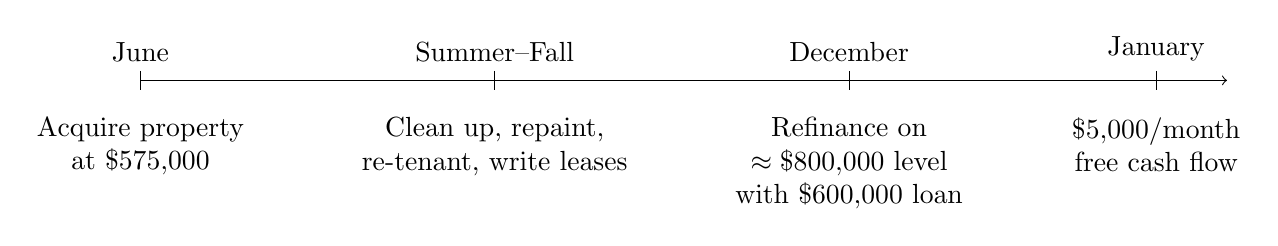
\begin{tikzpicture}[x=3.0cm,y=1cm]
\draw[->] (0,0) -- (4.6,0);
\foreach \x in {0,1.5,3.0,4.3}
  \draw (\x,0.12) -- (\x,-0.12);

\node[align=center,above] at (0,0.12) {June};
\node[align=center,below] at (0,-0.35) {Acquire property\\at \(\$575{,}000\)};

\node[align=center,above] at (1.5,0.12) {Summer--Fall};
\node[align=center,below] at (1.5,-0.35) {Clean up, repaint,\\re-tenant, write leases};

\node[align=center,above] at (3.0,0.12) {December};
\node[align=center,below] at (3.0,-0.35) {Refinance on\\\(\approx \$800{,}000\) level\\with \(\$600{,}000\) loan};

\node[align=center,above] at (4.3,0.12) {January};
\node[align=center,below] at (4.3,-0.35) {\(\$5{,}000\)/month\\free cash flow};
\end{tikzpicture}
\caption{Transcript-based reconstruction of the first-property sequence: acquisition, operational improvement, refinance, and recurring cash flow.}
\end{figure}

\paragraph{Worked example.}
The lecture's internal arithmetic can be read in a disciplined way if we proceed step by step:
\begin{enumerate}
\item The initial acquisition requires essentially total personal commitment, since the bank balance after closing is said to be \(\$50\).
\item The asset is then improved operationally rather than magically: tenants are replaced, appearance is improved, leases are written, and the property is made legible to the market as a better asset.
\item The later refinance-related level is stated as roughly \(\$800{,}000\), and the associated loan is \(\$600{,}000\).
\item At the level of the purchase price alone, the refinance loan exceeds the original purchase price by \(\$25{,}000\):
\begin{equation}
L_1 - P_0 = \$600{,}000 - \$575{,}000 = \$25{,}000.
\end{equation}
\item This does \emph{not} by itself prove that all costs were recovered, because the lecture does not supply exact closing costs, improvement costs, or debt terms. But it does show why the speaker can plausibly say that the capital was pulled back out after the property was improved.
\item From January onward, the asset is described as producing \(\$5{,}000\) per month in free cash flow, so the mechanism has changed from one-time gain to recurring income.
\end{enumerate}

The lecture's claim is therefore not just that risk paid off. It is that operational work changed the character of the asset fast enough to refinance it, recover capital, and leave a recurring income stream in place. That is the first full economic argument of the interview.

\section{Books, First Principles, and the Real-Estate Thesis}

After the first-property case study, the lecture expands again. The speaker turns to books, first mentioning Tony Robbins as an early motivational force and then generalizing to a wider reading discipline: when one reads practitioners, one is buying access to decades of compressed experience.

That reading discussion then becomes a hinge. The interviewer asks for the top three takeaways from Napola's own book, and the lecture uses that question to restate its central doctrine in a more organized form. The first takeaway is the strongest thesis of the chapter: across sectors, great fortunes continue to allocate into real estate.

\begin{figure}[h]
\centering

\includegraphics[width=0.82\textwidth]{lecture_110_figure_03.png}
\caption{On-screen emphasis for the lecture's central thesis: major fortunes, whatever their original industry, continue to allocate into real estate.}
\end{figure}

The lecture then turns that slogan into a retirement heuristic. We are not being told that one property makes everyone rich. We are being told that a single correctly chosen and steadily held asset can alter the geometry of later life:
\begin{equation}
T_{\text{payoff}} \approx 20\text{--}25\ \text{years}
\quad \Rightarrow \quad
\text{one owned property can become a retirement base.}
\end{equation}

The second takeaway is a classification problem: not every property type fits every operator. If one has time and appetite for active improvement, value-add property may be appropriate. If one has a demanding outside profession, that same property may be a bad fit. The third takeaway is a pedagogical claim: commercial property is more accessible than most people think, provided that one learns the business and begins with something one can manage.

At this stage the lecture has widened from one entrepreneur's anecdote into a general picture:
\begin{enumerate}
\item real estate is where major pools of capital repeatedly settle,
\item even one correctly handled asset can matter over decades,
\item property choice must fit the operator's actual life,
\item the field is less inaccessible than it appears from a distance.
\end{enumerate}

\section{Entry, Capital, and the Scarcity of Good Deals}

The next beat is the clearest tension in the lecture. The interviewer raises the common obstacle directly: many people assume that without large personal capital they simply cannot buy property. Napola's answer is not a motivational slogan. It is a reversal of what is scarce.

\subsection{Question \& Answer}

\paragraph{Question.}
How can someone with little money, little credit, and no obvious balance-sheet strength still enter real estate?

\paragraph{Answer.}
The lecture answers by shifting attention from capital to deal quality. Napola invokes a local example, Aventura Mall, and says in effect: if a sufficiently valuable property were offered at a sufficiently low price, money would appear. The lecture's point is heuristic, but it can be written compactly:
\begin{align}
V_{\text{mall}} &\approx \$3\times 10^9, &
P_{\text{hyp}} &= \$1\times 10^9.
\end{align}
The gap is not offered as a literal transaction forecast. It is a thought experiment meant to isolate the scarce object. If the deal is extraordinary, the financing problem changes character:
\begin{equation}
D_{\text{good}} \Rightarrow K_{\text{outside}}\ \text{is easier to source.}
\end{equation}

We should read this carefully. The lecture is not claiming that capital constraints do not exist. It is claiming that beginners frequently misidentify the bottleneck. The truly hard thing is to locate, understand, and control a good deal. Money can then be recruited behind that deal. In the lecture's language, money is easier than the deal.

This inversion is central enough to deserve a short logical chain:
\begin{enumerate}
\item most beginners think the missing object is cash,
\item the lecture says the missing object is an unusually strong opportunity,
\item strong opportunities attract lenders, investors, and experienced operators,
\item therefore entry begins with the search for the deal, not with despair over the personal balance sheet.
\end{enumerate}

\section{Operating Edge, Local Radius, and Going Against the Grain}

Once the entry problem is reframed, the lecture turns to edge. The question is no longer simply how to begin. It is how to compete.

Napola's answer is operational and local. The firm does not scatter itself across the country. It keeps the portfolio within a radius that permits direct observation, quick intervention, and repeated contact with the actual assets:
\begin{align}
R &\approx 250\text{--}300\ \text{miles}, &
A_{\text{deal}} &= 165{,}000\ \text{sq ft}, &
P_{\text{deal}} &= \$25{,}000{,}000.
\end{align}
The radius \(R\) is not decorative. It defines a region in which the owner can inspect properties, understand tenants, coordinate leasing, accounting, and management, and exploit synergies across nearby assets. The lecture is very explicit that in-house control matters. The same people talk to one another. One tenant base informs another. Knowledge circulates inside the firm rather than leaking out to a loose network of outside vendors.

The later large deal, bought for \(\$25\) million and described as 165,000 square feet of shopping centers built over a ten-year span, serves as the institutional-scale version of the earlier lesson. The business still buys by understanding ownership structure, local conditions, and opportunity. Scale changes, but the method does not.

From there the lecture makes one last strategic move: it warns against herd thinking. The real-estate market, like every other market, produces fashionable panic and fashionable enthusiasm. Napola's rule is to go against the grain. When everyone is terrified, one should at least ask whether assets are being mispriced downward. When everyone is aggressive, one should ask whether discipline is dissolving.

This is not formal market timing in an econometric sense. It is a principle of selective nonconformity. The lecture keeps it qualitative because it is meant as a decision rule, not a theorem.

The closing stretch then turns from market behavior back to personal structure. Why do we want wealth? If the answer is display, the lecture predicts failure. If the answer is financial freedom, family stability, and freedom from monthly fear, then the long project can hold. The final resilience claim follows naturally: even if the bank account were driven to zero, the operator's real capital now consists of knowledge, reputation, contacts, and repeatable pattern recognition. That is why the speaker says he would return to real estate immediately if he had to rebuild.

\section{Summary}

The lecture moves from biography to mechanism with unusual economy. First it establishes authority. Then it identifies the weakness of commission-dependent income. Then it shows how mentorship, discipline, and a willingness to act can compress years of uncertainty. The first-property case supplies the chapter's main arithmetic: acquire, improve, refinance, recover capital, and hold for cash flow. The later sections widen that case into doctrine: real estate remains a destination for large pools of capital, the true scarcity is the good deal rather than the money, local operational control is a real edge, and long-run wealth depends at least as much on the structure of our assets and motives as on the size of any single paycheck.